\subsection{x86}

\subsubsection{MSVC}

\RU{Компилируем}\EN{Let's compile}:

\lstinputlisting[caption=MSVC 2008]{patterns/13_arrays/1_simple/simple_msvc.asm}

\index{x86!\Instructions!SHL}
\RU{Ничего особенного, просто два цикла. Один изменяет массив, второй печатает его содержимое. 
Команда \INS{shl ecx, 1} используется для умножения \ECX на 2, об этом ниже~(\myref{SHR}).}
\EN{Nothing very special, just two loops: the first is a filling loop and second is a printing loop.
The \TT{shl ecx, 1} instruction is used for value multiplication by 2 in \ECX, more about below~\myref{SHR}.}

\RU{Под массив выделено в стеке 80 байт, это 20 элементов по 4 байта.}
\EN{80 bytes are allocated on the stack for the array, 20 elements of 4 bytes.}

\ifdefined\IncludeOlly
\clearpage
\RU{Попробуем этот пример в}\EN{Let's try this example in} \olly.
\index{\olly}

\RU{Видно, как заполнился массив}\EN{We see how the array gets filled}: 
\RU{каждый элемент это 32-битное слово типа \Tint, с шагом 2:}
\EN{each element is 32-bit word of \Tint type and its value is the index multiplied by 2:}

\begin{figure}[H]
\centering
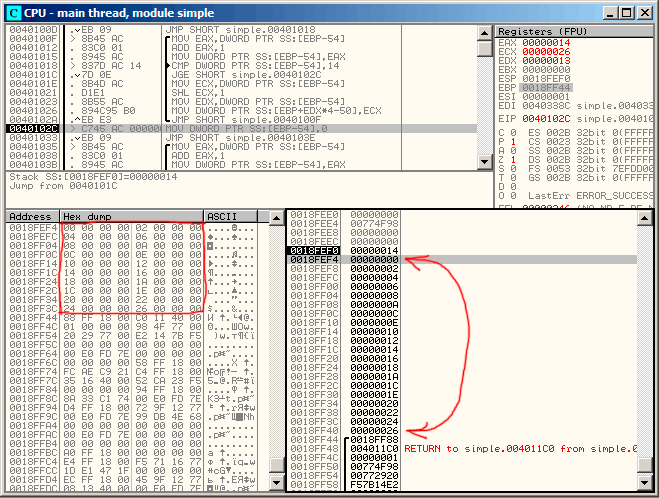
\includegraphics[scale=\FigScale]{patterns/13_arrays/1_simple/olly.png}
\caption{\olly: \RU{после заполнения массива}\EN{after array filling}}
\label{fig:array_simple_olly}
\end{figure}

\RU{А так как этот массив находится в стеке, то мы видим все его 20 элементов внутри стека.}
\EN{Since this array is located in the stack, we can see all its 20 elements there.}

\fi

\ifdefined\IncludeGCC
\subsubsection{GCC}

\RU{Рассмотрим результат работы GCC 4.4.1:}\EN{Here is what GCC 4.4.1 does:}

\lstinputlisting[caption=GCC 4.4.1]{patterns/13_arrays/1_simple/simple_gcc.asm}

\RU{Переменная $a$ в нашем примере имеет тип \IT{int*} (указатель на \Tint{}).
Вы можете попробовать передать в другую функцию указатель на массив,
но точнее было бы сказать, что передается указатель на первый элемент массива
(а адреса остальных элементов массива можно вычислить очевидным образом).}
\EN{By the way, variable $a$ is of type  \IT{int*} 
(the pointer to \Tint{})---you can pass a pointer to an array to another function,
but it's more correct to say that a pointer to the first element of the array is passed
(the addresses of rest of the elements are calculated in an obvious way).}
\RU{Если индексировать этот указатель как \IT{a[idx]}, \IT{idx} просто прибавляется к указателю 
и возвращается элемент, расположенный там, куда ссылается вычисленный указатель.}
\EN{If you index this pointer as \IT{a[idx]}, \IT{idx} is just to be added to the pointer 
and the element placed there (to which calculated pointer is pointing) is to be returned.}

\RU{Вот любопытный пример. Строка символов вроде \IT{\q{string}} это массив из символов. 
Она имеет тип \IT{const char[]}.}\EN{An interesting example: a string of characters like 
\IT{\q{string}} is an array of characters and it has a type of \IT{const char[]}.}
\RU{К этому указателю также можно применять индекс.}
\EN{An index can also be applied to this pointer.}
\RU{Поэтому можно написать даже так:  \TT{\q{string}[i]}~--- это совершенно легальное выражение в \CCpp!}
\EN{And that is why it is possible to write things like \TT{\q{string}[i]}---this is a correct \CCpp expression!}
\fi
